\documentclass[final,5p,times,twocolumn]{elsarticle}
\usepackage{amssymb}
\usepackage[utf8]{inputenc} % charset do texto (utf8, latin1, etc.)
\usepackage[T1]{fontenc} % encoding da fonte (afeta a sep. de sílabas)
\usepackage{graphicx}
\usepackage{tabularx}
\usepackage{tcolorbox}
\graphicspath{ {Images/} }

\journal{Information and Software Technology}

%=======================================================================
% Início do documento.
%=======================================================================
\begin{document}

\begin{frontmatter}

\title{Microservices: A Survey of performance metrics and scalability}

\author[Unisinos]{Igor Fontana de Nardin\corref{cor1}}
\ead{igor.fdn@gmail.com}

\author[Unisinos]{Rodrigo da Rosa Righi}
\ead{rrrighi@unisinos.br}

\author[Unisinos]{Cristiano André da Costa}
\ead{cac@unisinos.br}


\address[Unisinos]{Universidade do vale do Rio dos Sinos, São Leopoldo, Brazil}
\cortext[cor1]{Corresponding author}

%=======================================================================
% Resumo
%=======================================================================
\begin{abstract}
Microservice is a new trend in software engineering that based on divide an application into several services, each one with a small function. This concept allows that programmers write the source code of each microservice using the better language and framework based on the microservice function. Several articles define and implements a microservice architecture and perform a performance and scalability evaluation, but few articles consolidate the information of these evaluations. It is essential this consolidation because the microservice is a growing structure and needs a literature review. Therefore, this article is a survey that aims to find the tendencies in microservice applications. First, we present a brief background explaining cloud computing and microservice. Microservice is perfect for cloud computing, and this section explains why. After that, we explain the method of our research. So, we defined six research questions that aim to identify the motivation for this evaluation, metrics used in microservice evaluation, the application classes of microservice, the distributed system used to improve the application, and the communication patterns and protocols to microservice. These research questions guide the search string to find the articles to our survey. We applied this search string into some electronic databases. With the result of this search, we answered the research questions and proposed a taxonomy to direct future implementations. After that, we explain some tendencies and opportunities to microservice adoption.
\end{abstract}

\begin {keyword}
Microservices \sep Performance \sep Scalability \sep Metrics \sep Quality of service
\end{keyword}

\end{frontmatter}

%=======================================================================
% Introdução
%=======================================================================
\section{Introduction}
\label{intro}
At the beginning of software development, the developers implemented their software with the monolithic approach. In this approach, a single executable compacts all functionalities. Therefore, even if the user only needs one function, he will receive all the functions package of that software. When this application is on the internet, can be difficult to improve performance. For example, one function has an increase in its requisitions, so, to provide performance and scalability, the system needs to add more software instances. In the monolithic approach, the new instance replicates all the application, when only part of the application was required. An evolution of this approach is microservice architecture.

Big companies, like Netflix, Amazon, and The Guardian use the microservice architectures in their solutions ~\cite{Francesco2017ResearchAdoption}. In the microservice architecture, the developer decomposes the software into a set of small services, each running in its process and using a lightweight mechanism to communication (like REST)~\cite{Fowler2014Microservices}. Each service has a clear function and performs just this function, and because of this definition that microservice has this nomenclature. Decomposing the software allows that each microservice use the better framework to implements its purpose. For example, the programmer can use the Java language to implements a user interface microservice and R language to process complex calculations. Besides that, this decomposition enables the scaling of just one software microservice. So, if one microservice has an increase in its requisitions, just this microservice will replicate to a new instance.

A microservice architecture facilitates the adjustments in the functions, but this approach will not make these improvements by itself. The software manager needs to analyze and decide when adjusting the application environment. Decide the best moment to improve the application is not an easy decision. For example, a web application can have a peak moment of usage. Make a decision based only on this peak can instantiate a resource inappropriately. Besides that, if the manager takes too long to instantiate a new resource when an undesirable state reaches may affect the application performance. Therefore, it is essential to describe some architectures, metrics, patterns, and protocols for microservice performance and scalability bias.

Some articles aim to demonstrate some tendencies and opportunities to microservice. In~\cite{Almeida2017SurveyEnvironment} the authors presented a survey about microservice architecture focusing on security, privacy and standardization aspects. This article analyzes just microservices in cloud computing environments. Already the article~\cite{Francesco2017ResearchAdoption} consists of a systematic mapping study in three perspectives: publication trends, the research focus, and potential for industrial adoption. Like~\cite{Almeida2017SurveyEnvironment}, in~\cite{Yu2018AApplications} the primary motivation is security, but in this article, the focus is on the communication between microservices. This article presents some concerns about microservice communication and in the end, demonstrate an ideal solution for security issues. The article~\cite{Alshuqayran2016AArchitecture} presents a systematic mapping study to find architectural challenges, architectural diagrams/views, and quality attributes. Finally, the article~\cite{Cerny2018ContextualArchitecture} presents a systematic mapping study to identify interest and challenges in microservices. 

None of the above articles focus on microservice performance and scalability or how to improve this. Therefore, this survey aims to present update review about tendencies and opportunities for microservice performance and scalability. So, we define research questions to find motivations, metrics, algorithms, application classes, architectures, and communication patterns and protocols about microservice evaluation. With the results, we proposed a taxonomy to direct future implementations in microservices. Therefore, we will show some tendencies and opportunities found in the reviewed articles.

The rest of this paper is structured as follows: Section~\ref{background} explains some concepts about microservice and cloud computing (the major microservice case). Section~\ref{methods} explains the research method that we use in this study. Section~\ref{results} shows the results of our research. In section~\ref{Discussion}, we present a discussion about the tendencies of microservice performance and scalability. Section~\ref{opportunities} demonstrates some opportunities for future works in microservice that we did not find in our research. Finally, in section~\ref{conclusion} we conclude and present future studies.

%=======================================================================
% Fundamentação teórica
%=======================================================================
\section{Background}
\label{background}
In this section, we will explain some concepts that are the base for our research. Before presenting microservice, we will detail the cloud computing, a distributed system that allows the utilization of microservice architecture. After introducing cloud computing, we explain the concepts about microservice, like communication patterns and the relationship with SOA (service-oriented architecture).


%Cloud computing
%%O que é?
%%Modelos de serviço
%%Middlewares de cloud
%%Características essenciais (NIST)
%%Elasticidade
%%%Definição
%%%Tipos de elasticidade
%%%Forma de tratamento da elasticidade

%Microserviços
%%Definição e engenharia de software
%%Características
%%Diferença entre microserviços e orientado a serviços

\begin{figure*}[ht]
\centering
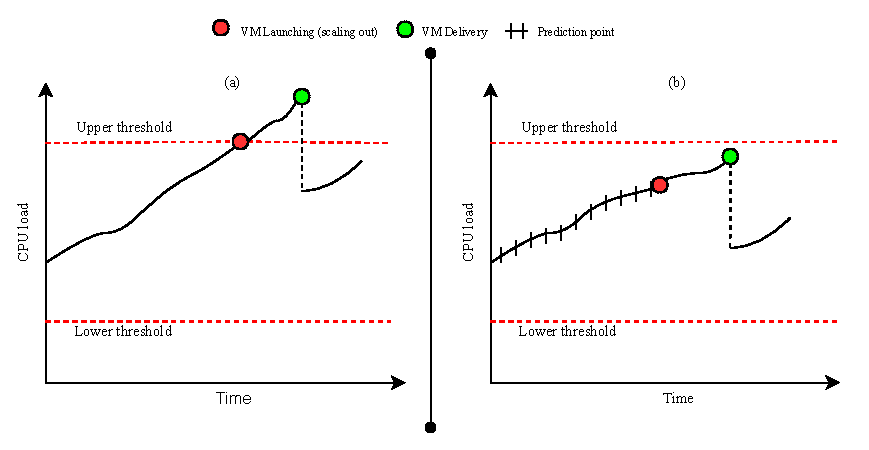
\includegraphics{Images/Previsto_real.pdf}
\caption{Elasticity approaches: (a) reactive; (b) proactive.}
\label{previsto}
\end{figure*}

%=======================================================================
% Fundamentação teórica - Cloud computing
%=======================================================================
\subsection{Cloud computing}
The network technologies improvements have proportioned reliable and high-speed access to remote resources over the Internet. These improvements have brought the idea of centralized processing to large data centers around the world, rather than running locally \cite{Marinescu2013CloudPractice}. On the other hand, this approach increased the resources sharing through the network, initially using grids and recently through Cloud computing \citep{Marinescu2013CloudPractice}.

Cloud computing is a paradigm that provides a ubiquitous network that can adjust computing resources and can quickly provisioned and released with minimal management effort or interaction with the service provider \cite{Mell2011TheComputing}. Previously, Cloud computing used as a strictly academic term. However, in recent years cloud computing appears in the most diverse services types provided over the Internet (often without the user knowing) \cite{Marinescu2013CloudPractice}.

The services models, presented by \cite{Mell2011TheComputing}, evidenced the cloud impact on early 21st-century society. Currently, \cite{Mell2011TheComputing} presents three service models:

\textbullet\ Software as a Service (SaaS): User uses an application deployed in the cloud. All the infrastructure is maintained by those who deployed the application, and the user does not manage or control the environment resources \cite{Mell2011TheComputing};

\textbullet\ Platform as a Service (PaaS): Provides an environment ready for application development. Just like in SaaS, who provides the service maintain the environment, but the user has control over the deployed applications. A PaaS example is a virtual machine configured on a server, which has the entire framework to develop Python applications \cite{Mell2011TheComputing};

\textbullet\ Infrastructure as a Service (IaaS): The cloud provider gives the infrastructure for users. Therefore, it is possible to develop or run any application, having access and control over the environment, such as network, operating system, storage, and CPU \cite{Mell2011TheComputing};

Applications like email servers (such as Gmail) are a SaaS classic example. Users do not have access to the cloud settings in which the application is running, and they only have access to the application's settings. In PaaS, we have some examples, like Pythonanywhere, service that provides a cloud environment ready for Python applications development. Finally, IaaS provides a more customizable environment, allowing network configuration, operating system definition, storage, and CPU. 

In extension to the service model, cloud computing has three deployment models, which relate to how to access these services \cite{Mell2011TheComputing}:

\textbullet\ Private cloud: Clouds provided for a specific use of an organization. Maintained by the organization, by a provider or by a mixture of the two previous ones. Typically, the cloud is in a restricted environment, without the data being available to an unregistered user;

\textbullet\ Public cloud: They are clouds managed by a provider, which provides all the infrastructure. A significant concern in this deployment model is that the provider has access to all the data storage in the cloud. On the other hand, it facilitates applications deployment without significant investments in their infrastructure;

\textbullet\ Hybrid cloud: It is a private and a public cloud combined. Hybrid is relevant in situations where an organization has a cloud (private) infrastructure but may need more resources from a public cloud.

%%Middlewares de cloud
To provide these models, several middlewares that act as the cloud manager, acting at the IaaS level. Several management tools are open source and enable Private clouds or Hybrid clouds creation. Some Open-Source middlewares examples are OpenNebula \cite{Moreno-Vozmediano2012IaaSInfrastructures}, Eucalyptus \cite{Nurmi2009TheSystem}, and OpenStack \cite{Sefraoui2012OpenStack:Computing}. An essential public clouds feature is the pay-as-you-go concept, which consists of charging the user for the usage time and the amount of resources allocation.

Any cloud management middleware provides an application programming interface (API), additionally to a graphical or command line interface. With this API, anyone can develop applications that monitor and manage features according to users needs and application behavior. Several academic examples use the API to develop solutions, such as \cite{DaRosaRighi2016Autoelastic:Cloud}, \cite{Molto2013ElasticRequirements}, \cite{Spinner2014RuntimeEstimation}, \cite{Beernaert2012AutomaticOpenStack}, \cite{Roy2011EfficientForecasting}, \cite{Loff2014Vadara:Applications}, and \cite{Rosa2014AnMechanisms}.

Cloud computing is only possible due to resources virtualization through virtual machines (VMs). VMs can perform the same computational functions that a physical computer \cite{Birman2012GuideSystems}. Typically, exists data centers that allow allocating multiple virtual machines according to the user needs \cite{Marinescu2013CloudPractice}. This virtualization provides some benefits over the predecessor multicomputers, like clusters and grids. The first one is simplified management, requiring few managers to set up and release new features \cite{Birman2012GuideSystems}. Through access interfaces (graphical, command line or programming), it is possible to adjust virtual machine configurations, such as memory, CPU, and others. In comparison to physical media, changing some of these settings requires buying hardware and spending hours installing and configuring \cite{Birman2012GuideSystems}.

Another strong point of cloud computing is green computing. With the right Cloud computing management it is possible to keep active only the needed VMs \cite{Righi2013ElasticidadeDesafios}. Besides, cloud servers are optimized. They use less energy cost compared to physical machines with similar resources.

Until then, anything is different from something already presented in another distributed systems. The high differential of the cloud computing model is the elasticity \cite{Righi2013ElasticidadeDesafios}.

%%Elasticidade
\begin{figure*}[ht]
\centering
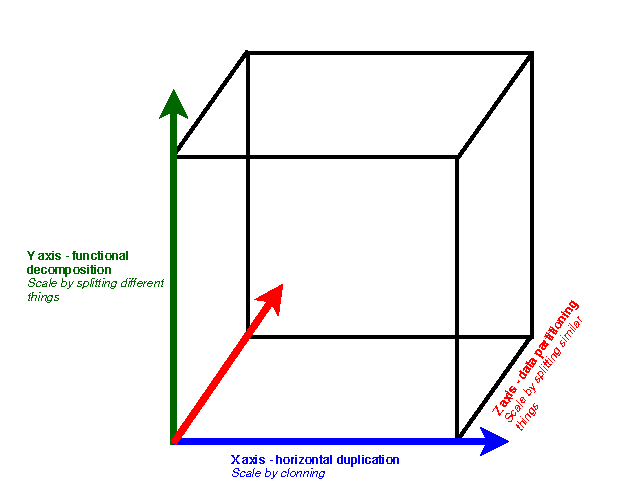
\includegraphics{Images/ScaleCube.pdf}
\caption{Scale cube \cite{MartinL.Abbott2015TheLivros}}
\label{scaleCube}
\end{figure*}


\subsection{Elasticity}

%%%Definição
Elasticity is one of the most significant cloud computing features \cite{Molto2013ElasticRequirements}. Elasticity is the ability to adapt the resources on the fly according to need. There are two types of elasticity in cloud computing \cite{Righi2013ElasticidadeDesafios}. 

%%%Tipos de elasticidade
The first one is horizontal elasticity, which quickly provisions and releases computational nodes (virtual machines)  \cite{Molto2013ElasticRequirements}. This elasticity is frequently used to adjust cloud according to changes in workload and to avoid additional costs. For example, there is a virtual machine in charge of dealing with web requests. At a specific time of the day, the number of request increase and only one machine is not enough. Thus, by identifying this peak, the manager can (manually or automatically) instantiate new machines quickly.

The other elasticity form is vertical, which is the ability to adjust virtual machines settings, increasing or decreasing their capacity \cite{Spinner2014RuntimeEstimation}. In other words, vertical elasticity is the possibility to increase resources, such as CPU, memory, and network type, without the need for hardware changes. The weakness in this approach is that some middlewares, such as OpenNebula, require to turn off the virtual machine to adjust some of its parameters (such as CPU) \cite{Moreno-Vozmediano2012IaaSInfrastructures}.

Regardless of the elasticity type, this is a crucial element to improve application performance. For example, it is possible to add new virtual machines to perform tasks (horizontal elasticity) or increase some virtual machine resource (vertical elasticity) so that it can finish its task faster \cite{Righi2013ElasticidadeDesafios}. 

%%%Forma de tratamento da elasticidade
Resources allocation can follow two approaches \cite{Righi2013ElasticidadeDesafios}. The first one is the manual resources allocation, which requires user action. Public and private middlewares have tools to make these adjustments, usually through a graphical interface, command line or programming API \cite{Righi2013ElasticidadeDesafios}. The second approach is automatic and has two types of treatment: reactive and proactive \cite{Righi2013ElasticidadeDesafios}. 

In the reactive form, according to statically defined rules is to perform elasticity decisions. Commercial systems, such as Amazon AWS, Nimbus, and Windows Azure, use this way to provide elasticity \cite{Righi2013ElasticidadeDesafios}. The rules define metrics thresholds and the elasticity action to perform when thresholds reach. A cloud receives these rules through a Service Level Objective (SLO) \cite{Spinner2014RuntimeEstimation}. A reactive elasticity example is to indicate that if a virtual machine reaches 20\% CPU, it needs turning off (horizontal elasticity) or it must decrease its total CPU (vertical elasticity).

The cloud adapts according to the thresholds defined in SLO. However, reactive elasticity has two significant problems. The first one is how to define the best thresholds for a given application. This definition is not trivial and requires ability from user to configure management tool besides an analysis of each application separately \cite{Righi2013ElasticidadeDesafios}.

The second problem is that the reactive elasticity performs an action when a resource reaches an undesirable state (defined by the threshold). In horizontal elasticity, after triggering the adding a new resource action, there is an interval to starts this resource. Then, after reaching an undesirable state, it will remain in that state until the new feature is ready. This time varies for each cloud manager, VM size,  and host hardware, but some authors indicate that the virtual machine instantiation time is between 5 and 15 minutes \cite{Bankole2013CloudEnvironment, Brebner2012IsEnough}.

The proactive approach aims to solve the reactive problems (mainly, the second one). This approach used historical data to detect patterns and to predict the best time to act \cite{Righi2013ElasticidadeDesafios}. Thus, the forecast uses the resource initialization time and this smooth the violation problem. Machine learning or time series calculations are the algorithms usually used for this prediction \cite{Rosa2014AnMechanisms, Gong2010PRESS:Systems, Loff2014Vadara:Applications, Roy2011EfficientForecasting, Moore2013TransformingAuto-scaling, Barrett2013ApplyingCloud, Nikravesh2017AnProvisioning}. Figure~\ref{previsto} demonstrates the reactive and proactive behaviors. In (a) exemplifies how the CPU of a system could behave in the reactive form. A VM launch when CPU reaches a threshold. The CPU stays in an undesirable state until the VM is ready. In (b) exemplifies the proactive approach. The system predicts that will be necessary to instantiate a new virtual machine. Then, the manager instantiates a new resource to deal with CPU peak. When the virtual machine is ready generates a CPU smoothing. 

\begin{figure*}[th]
\centering
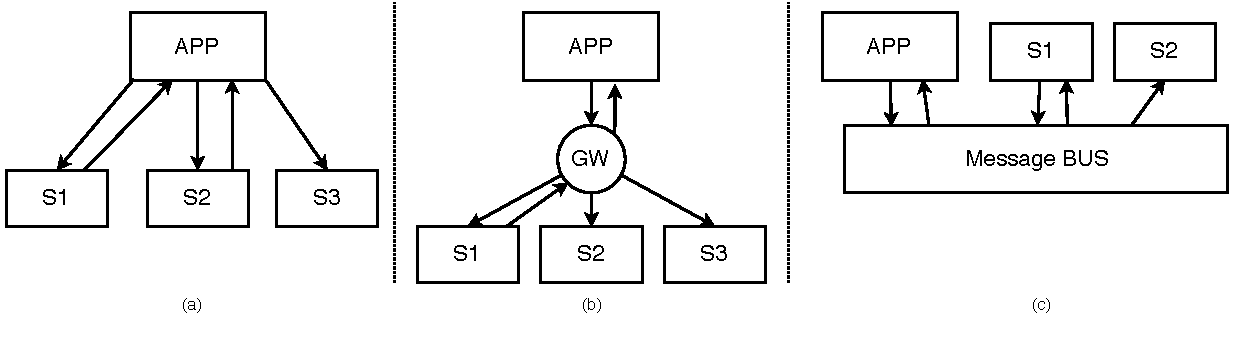
\includegraphics[scale=0.8]{Images/Microservices_comm.pdf}
\caption{Patterns of communication through microservices \cite{Namiot2014OnArchitecture}. (a) The application communicates directly with the services. (b) The gateway receives the requisition and passes it to the appropriate microservice. (c) Message bus where the application and services communicate through it.}
\label{microcomm}
\end{figure*}

As mentioned earlier, a web server is an example of the use of elasticity, which, according to the workload, adds more VMs to handle the requests increase. This approach is a classic example of elasticity that uses the replication strategy \cite{Righi2013ElasticidadeDesafios}. In this strategy, there is a pre-configured virtual machine template of application. This template is used to create a new virtual machine when necessary. Typically, the replicated machines do not communicate with each other, but through a centralizer that distributes tasks \cite{Righi2013ElasticidadeDesafios}. Also, these machines can exchange information through shared memory. In addition to web applications, high-performance applications, such as those following the master-slave model, can use the replication approach \cite{Righi2013ElasticidadeDesafios}.

Besides the above strategy, two others can be used to provide elasticity \cite{Righi2013ElasticidadeDesafios}. The first is resource migration, which consists of migrating VMs between physical resources. Regarding performance, several middlewares allow this migration in acceptable terms, and this strategy is particularly interesting concerning energy consumption \cite{Righi2013ElasticidadeDesafios}. It is possible to join virtual machines of different physical resources, allowing resources disconnection.

Finally, the last is the resizing strategy. An example of this strategy is to adjust the percentage of CPU used by a virtual machine so that it finishes its processing faster. Resizing is not exclusive to CPU, for example, this could also adjust the bandwidth of a virtual private network \cite{Righi2013ElasticidadeDesafios}. Not all cloud computing middlewares enable on-the-fly scaling, requiring virtual machine shutdown before resizing. Regarding high-performance applications, this is particularly critical as it would require a time-out, resizing, and initialization.

Elasticity can improve the performance of a large variety of applications type submitted to the cloud. However, an architecture approach is growing its utilization combined with a cloud. This approach is microservice.

%=======================================================================
% Fundamentação teórica - Microserviços
%=======================================================================
\subsection{Microservices}

%Intro
The most traditional architecture to develop an application, independent of the application purpose, is monolithic. In small applications, this architecture has several advantages, such as simplicity of development, testing and deploying \cite{Chen2017FromApproach}. However, as applications increase and grow complexity, these advantages tend to become disadvantages. For example, implement new features without inserting bugs becomes more complicated, since the developer does not know all the impact of their changes. 

Another limitation of large monolithic applications is scalability \cite{Chen2017FromApproach}. For example, to handle an increase in requests a cloud needs invoke more instances of the application. In monolithic, the entire application needs to replicate. However, perhaps only a part of the applications needs to replicate.

%%Motivação
To mitigate these disadvantages, an approach that is increasing followers, both academia and industry, is the architecture based on microservices ~\cite{Chen2017FromApproach}. Microservices consists of developing an application creating several small and independent services \cite{Namiot2014OnArchitecture}. 

This development approach has grown in recent years but is not something new. The term microservices has emerged in the agile development community since 2014 \cite{Zimmermann2017MicroservicesDeployment}. Some authors consider Microservices as a new approach to the Service-Oriented Architecture (SOA) architecture, which primarily consists of dividing an application into services ~\cite{Zimmermann2017MicroservicesDeployment}. However, there is no agreement on the relationship between microservices and SOA \cite{Chen2017FromApproach}.

%Definição e engenharia de software
This architecture consists of a set of small services with the least possible responsibility. In other words, a service has a well-defined function in the system. These services communicated through a lightweight protocol (such as HTTP) \cite{Namiot2014OnArchitecture}. So, unlike the monolithic approach which has an application only, in microservices we have several separate services that can communicate with each other. These services do not have to be written in the same programming language, allowing implement the best strategy for each new service.

%%Comparação com monolítico
Thus, an architecture based on microservices becomes attractive in comparison to monolithic architectures for several reasons. Developing new features becomes simple since the scope of the service is well-defined with little coupling between services. In monolithic applications, there is usually a high coupling between classes \cite{Namiot2014OnArchitecture}. 

Another consideration for the comparison between these two architectures is the scalability. The scale cube, shown in figure~\ref{scaleCube}, describes the approaches to provide scalability to an application \cite{Namiot2014OnArchitecture}. At the start point, there is a monolithic application with no scalability. A monolithic application can scale by adding new replicas of the application, represented in figure~\ref{scaleCube} as the X-axis.

Another way to provide scalability can be by splitting the data of an application. In this way, each server runs an identical application, but each one is responsible for a part of the data \cite{Namiot2014OnArchitecture}. An example of this is database sharding, which consists in using the primary key of a table to data routing \cite{Namiot2014OnArchitecture}. The z-axis in figure~\ref{scaleCube} exemplifies this scalability

Adding new replicas or splitting the data can increase the scalability of the monolithic application without performing a decomposition of services, but this can increase the complexity of the system \cite{Namiot2014OnArchitecture}. While data decomposition split similar things, decomposing functions divide a large system into smaller (micro) services that do different things \cite{Namiot2014OnArchitecture}. Thus, a monolithic application becomes a set of small services, and the scaler manager can replicate these services individually.

These concepts can be applied in combination, aiming at a better performance of the application. For example, the developer can divide a large application into several microservices, applying functional decomposition. While in a monolithic system a requisition executes the entire application, with the decomposition, the requisition performs just the required service.  This division could be enough to increase the performance and scalability of the system, but If it is not enough, the developer can combine the replication of a critical service.

While in monolithic systems communication is not critical, in microservices, just like any distributed system, it becomes a crucial point. Services are in constant communication with each other and with external applications. The figure~\ref{microcomm} shows three communication patterns \cite{Namiot2014OnArchitecture}. 

In (a) we have an application communicating directly with the services, without any intermediary. This approach offers a simple implementation and management. However, when it is necessary to apply the replication of some services, it will be necessary to modify the application and services. This modification becomes necessary because there is no load balancer to route the application request to the correct service. Also, both the application and the services must use the same communication protocol. The communication protocol can be a significant problem because the services are heterogeneous, requiring the application to implement all the communication protocols of the services it wants to communicate. Usually, services implement the HTTP protocol.

Thus, the pattern (b) of figure~\ref{microcomm} that, unlike the previous model, adds a gateway between applications and services \cite{Namiot2014OnArchitecture}. The gateway knows the protocol of all the services of its system, giving to the applications a unique communication protocol. Besides, the gateway rotates the requests for services. With this routing, the system can add new nodes without changing applications and services.

Another pattern of communication is presented in (c), where there is a single communication bus used by both applications and services. Like the previous model, this model also enables the replication of services, but the services need to verify which requests are their responsibility. Also, there must be a way to indicate that a service is processing a request, so that two microservices do not process the same thing.


%=======================================================================
% Seleção dos artigos
%=======================================================================
\section{Methods}
\label{methods}
\begin{table*}[htbp]
\centering
\renewcommand{\arraystretch}{1.5}
\caption{Research questions.}
\label{table_questions}
\begin{tabularx}{\textwidth}{ll@{\hspace{8em}}l}
\hline
\multicolumn{2}{l}{Group and identifier} & Issue \\ \hline
\multicolumn{2}{l}{\textbf{General questions (GQ)}} &  \\
 & CG1 & How would the microservice performance and scalability appear? \\
 & CG2 & What are the motivations to analyze and improve microservice? \\
\multicolumn{2}{l}{\textbf{Specific questions (SQ)}} &  \\
 & SQ1 & Which are the metrics and algorithms used to evaluate microservice? \\
 & SQ2 & Which are microservice applications classes? \\
 & SQ3 & What are the distributed system architecture of microservice applications? \\
 & SQ4 & Which are communication patterns and protocols to microservice? \\ \hline
\end{tabularx}
\end{table*}

After introducing cloud computing and microservices, we explain our study protocol to provide an overview of performance and scalability in microservices. We performed a systematic literature review following widely recognized guidelines \cite{Petticrew2006SystematicSciences} to plan and run systematic mapping studies. We choose this method to find technologies regarding microservices to perform performance and scalability, besides metrics that evaluate this.

First, in this section, we introduce the research questions that drive our review in subsection~\ref{questions}. After that, we present in subsection~\ref{search}, our search strategy and libraries explored to collect data. Then, in subsection ~\ref{selection} we demonstrate the criteria for selecting the studies, and in~\ref{data_extraction} we describe how we extract the data from the studies. Finally, in subsection~\ref{quality_assessment} we describe the quality assessment of the selected studies.

\subsection{Research Questions}
\label{questions}
According to \cite{Petticrew2006SystematicSciences}, the first and most important part of a systematic review is defining the right research questions. This definition will direct the entire research. Our focus is finding works that address performance and scalability in microservice applications. We seek for problems, challenges, metrics, and patterns that aim to improve and evaluate these applications.


We divide our research questions into two categories: general question (GQ) and specific question (SQ). Table~\ref{table_questions} lists all the research questions investigated.

The General Questions group of research questions involves a broader classification and some challenges concerning microservice performance and scalability. CG1 refers to how performance and scalability appear in related works. This question will contribute to creating a taxonomy in section~\ref{Discussion}. This research question highlights the technologies to provide performance and scalability.

GQ2 refers to the key challenges and issues in microservice performance and scalability. This question is the main factor that will serve as a direct influence on this survey. The purpose is to identify in the literature the types of issues in performance and scalability to microservices. This question will contribute to identifying challenges that we explore in section~\ref{Discussion}.

From General Questions, we derived some specific questions (SQ group) to improve the study filtering process. These questions have been proposed to pinpoint questions surrounding performance and scalability to microservices. From General Questions, we derived some specific questions (SQ group) to improve the study filtering process. These questions have been proposed to pinpoint questions surrounding performance and scalability to microservices. SQ1 seeks to identify the metrics used to evaluate performance and scalability in the microservices application. SQ2 investigates the classes of applications that usually applies microservices. SQ3 examines the types of distributed system architectures in microservice applications. SQ4 investigates the communication patterns and protocols to microservice.

\subsection{Search Strategy}
\label{search}
After defining the research questions, we propose the search strategy to find a complete set of studies related to the research questions. This process involved the designation of \textit{search keywords} and the \textit{definition of search scope} \cite{Petticrew2006SystematicSciences}. We defined keywords according to our research questions to obtain accurate search results. We used the PICO (population, intervention, comparison, and outcome) criteria that propose a guideline to define these keywords \cite{Akobeng2005PrinciplesMedicine.}. Follow these criteria allow us to find works that answer our research questions.

We defined PICO criteria based on the general research questions. We desire to refine and answer the specific research questions, which derived from the general research questions. Therefore, we defined the PICO criteria for microservice performance and scalability as follows.

\subsubsection{Population}
The populations involve keywords, related terms, variants, or the same meaning for the technologies and standards on microservice performance and scalability. Therefore, we created the following search string:

\begin{tcolorbox}[width=\linewidth,title={Search String},colbacktitle=white,coltitle=black]
("microservices" AND ("performance" OR "metrics" OR "quality of service" OR "scalability"))
\end{tcolorbox}

\subsubsection{Intervention}
We used the following terms to better filter studies in line with the purposes: microservices performance metrics, microservice architectures, scalability metrics, and classes of microservice applications. 

\subsubsection{Comparison}
This case refers to the comparison of different architecture types of microservice implementation that improve performance. Also, we compared applications metrics of microservice to evaluate performance. Besides, we compared the classes of the microservice application. 

\subsubsection{Outcome}
The outcomes related to factors of importance to application architect (e.g., improved performance) and the cloud administrator. These factors can refer to improving application response time, anticipating potential under/over provisioning, choosing the right metrics to evaluate the application, and choosing the better application architecture.

\subsection{Article Selection}
\label{selection}
In this section, we explain how we proceeded to remove the studies that were not relevant. We need to keep only articles that are the most representative in our research. Therefore, we removed the studies that did not address microservice performance and scalability specifically. So, we defined exclusion criteria to refine our search as follows:

\begin{itemize}
\item Exclusion criterion 1: the article does only address Internet of the Things architecture to microservice.
\item Exclusion criterion 2: the article does only address deploy of microservices.
\item Exclusion criterion 3: the article does only address the transformation of a monolithic application to a microservice application.
\end{itemize}

The steps of the filtering process are as follows: (1) impurity removal, (2) removal of duplicates, (3) filter by title, (4) filter by abstract, and (5) filter by full text.

First, we removed the impurities of the search results. This removal is essential because the search results include, for example, names of conferences correlated to the search keywords. 

Second, we grouped and removed duplicates of the articles because some studies were in more than one database.

Third and fourth, we analyzed the title and abstract of the articles and excluded those that did not address microservice performance and scalability as a subject.

Some studies remained that were not mainly related to this survey. We analyzed the full text to remove those that were not relevant.

\begin{table*}[tb]
\centering
\renewcommand{\arraystretch}{1.5}
\caption{Quality assessment criteria}
\label{table_quality}
\begin{tabularx}{\textwidth}{l@{\hspace{8em}}l}
\hline
Identifier & Issue \\ \hline
C1 & Does the article clearly explain the research purpose? \\
C2 & Does the article adequately describe the literature review, background, or context? \\
C3 & Does the article present the related work concerning the main contribution? \\
C4 & Does the article have an architecture proposal or research methodology described? \\
C5 & Does the article have research results? \\
C6 & Does the article present a conclusion related to the research objectives? \\
C7 & Does the article recommend future works, improvements, or further studies? \\ \hline
\end{tabularx}
\end{table*}
\begin{table*}[tb]
\centering
\renewcommand{\arraystretch}{1.5}
\caption{Review articles related to the research questions}
\label{table_extraction}
\begin{tabularx}{\textwidth}{ll@{\hspace{8em}}l@{\hspace{1em}}l}
\hline
\multicolumn{2}{l}{Section} & Description & Research questions \\ \hline

\multicolumn{2}{l}{\textbf{Open content}} &  &  \\
 & Title & Title of the scientific article & CG1, CG2, SQ1, SQ3 \\
 & Abstract & Summary of paper’s purpose, method, and results & CG1, CG2, SQ1, SQ3 \\
 & Keywords & Words representing the text content & CG1, CG2, SQ1, SQ3 \\
 
\multicolumn{2}{l}{\textbf{Article content}} &  &  \\
 & Introduction & Introduction specifies the issue to be addressed & All questions \\
 & Background & Section includes concepts and is related to the proposal & All questions \\
 & Method & Presents and describes the scientific methodology & All questions \\
 & Results & Performs an evaluation according to the proposed methodology & All questions \\
 & Discussion & Data that were quantified compared with the literature & All questions \\
 & Conclusion & Findings related to the objectives and hypotheses & All questions \\ \hline
\end{tabularx}
\end{table*}

\subsection{Quality assessment}
\label{quality_assessment}
Since it is essential to asses the quality of the selected studies, the quality criterion is intended to verify that the article is a relevant study \cite{Petticrew2006SystematicSciences}. For this purpose, we proposed Table~\ref{table_quality} with the questions that we apply to the selected studies to verify its quality. The questions of Table~\ref{table_quality} evaluated the selected articles concerning the purpose of research, contextualization, literature review, related work, methodology, the results obtained, and the conclusion according to objectives and indication of future studies.

\subsection{Data Extraction}
\label{data_extraction}
Finally, we created an evaluation scheme to gather information for the selected articles. This form indicates in which sections we search for answers to general and specific research questions. We presented this evaluation in Table~\ref{table_extraction}. This table supports us to understand how the studies have addressed the issues related to the proposed research questions.


%=======================================================================
% Estado da arte
%=======================================================================
\section{Results}
\label{results}
\begin{table*}[htbp]
\centering
\renewcommand{\arraystretch}{1.5}
\caption{List of articles.}
\label{table_articles}
\begin{tabular}{l@{\hspace{4em}}l@{\hspace{4em}}l@{\hspace{4em}}l@{\hspace{4em}}l}
\hline
Identifier & Study                                                                                                                                                      & Year & Publisher     & Type              \\ \hline
A01 & Gribaudo et al~\cite{Gribaudo2018} & 2018 & ScienceDirect & Journal \\
A02 & Kiss et al~\cite{Kiss2017} & 2017 & ScienceDirect & Newspaper Article \\
A03 & Pérez et al~\cite{Perez2018} & 2018 & ScienceDirect & Journal \\
A04 & Khomh et al~\cite{Khomh2018} & 2018 & ScienceDirect & Journal \\
A05 & Do et al~\cite{Do2017} & 2017 & IEEE & Conference \\
A06 & Kookarinrat et al~\cite{Kookarinrat2016} & 2016 & IEEE & Conference        \\
A07 & Zhang et al~\cite{Zhang2017} & 2017 & IEEE          & Newspaper Article \\
A08 & Lloyd et al~\cite{Lloyd2018} & 2018 & IEEE          & Journal           \\
A09 & Khazaei et al~\cite{Khazaei2017} & 2017 & IEEE          & Conference        \\
A10 & Klock et al~\cite{Klock2017} & 2017 & IEEE          & Conference        \\
A11 & Ueda et al~\cite{Ueda2016} & 2016 & IEEE          & Conference        \\
A12 & Patros et al~\cite{Patros2017} & 2017 & ACM           & Conference        \\
A13 & Alipour and Liu~\cite{Alipour2017} & 2017 & IEEE          & Conference        \\
A14 & Florio and Di Nitto~\cite{Florio2016} & 2016 & IEEE          & Conference        \\
A15 & Villamizar et al~\cite{Villamizar2015} & 2015 & IEEE          & Journal           \\
A16 & Shah et al~\cite{Shah2017} & 2017 & IEEE          & Journal           \\
A17 & Zhang et al~\cite{Zhang2017} & 2017 & IEEE          & Conference        \\
A18 & Moradi et al~\cite{Moradi2017} & 2017 & IEEE          & Conference        \\
A19 & Casalicchio and Perciballi~\cite{Casalicchio2017} & 2017 & IEEE          & Conference        \\
A20 & Toffetti et al~\cite{Toffetti2015} & 2015 & ACM           & Conference        \\
A21 & Julian et al~\cite{Julian2016} & 2016 & ACM           & Journal           \\
A22 & Suresh et al~\cite{Suresh2017} & 2017 & ACM           & Journal           \\
A23 & Khazaei et al~\cite{Khazaei2017} & 2017 & ACM           & Journal           \\
A24 & Barna et al~\cite{Barna2017} & 2017 & IEEE          & Conference        \\
A25 & Ben Hadj Yahia et al~\cite{BenHadjYahia2016} & 2016 & ACM           & Conference        \\
A26 & Gotin et al~\cite{Gotin2018} & 2018 & ACM           & Conference        \\
A27 & Klinaku et al~\cite{Klinaku2018} & 2018 & ACM           & Conference        \\
A28 & López et al~\cite{Lopez2017} & 2017 & ACM           & Conference        \\
A29 & Jenkins et al~\cite{Jenkins2017} & 2017 & IEEE & Conference        \\
A30 & Salah et al~\cite{Salah2017} & 2017 & IEEE          & Conference        \\
A31 & Singh et al~\cite{Singh2017} & 2017 & IEEE          & Conference        \\
A32 & Amaral et al~\cite{Amaral2016} & 2016 & IEEE          & Journal           \\
A33 & Al-Dhuraibi et al~\cite{Al-Dhuraibi2017} & 2017 & IEEE          & Journal           \\
A34 & Benchara et al~\cite{Benchara2017} & 2017 & IEEE          & Conference        \\ 
A35 & Higashino~\cite{Higashino2017ApplicationArchitecture} & 2017 & ACM          & Journal        \\ \hline
\end{tabular}
\end{table*}

In this section, we present the results obtained from the 35 fully assessed studies related to the research topic. We attempt to answer each proposed research question in the following subsections through elaborative information synthesis. After answering the research questions, we created an updated taxonomy with the state-of-the-art of applications microservice and how to improve scalability and performance. 

\subsection{Conducting the Search Strategy}
We selected 4 electronic databases as our search scope. We used ACM Digital Library, IEEE Xplore Library, ScienceDirect, and SciELO. These portals cover the most relevant journals and conferences within computer science. In the next subsection, we explain how we filter the studies. Figure~\ref{article_selection} shows our filtering process. 

\begin{figure*}[htb]
\centering
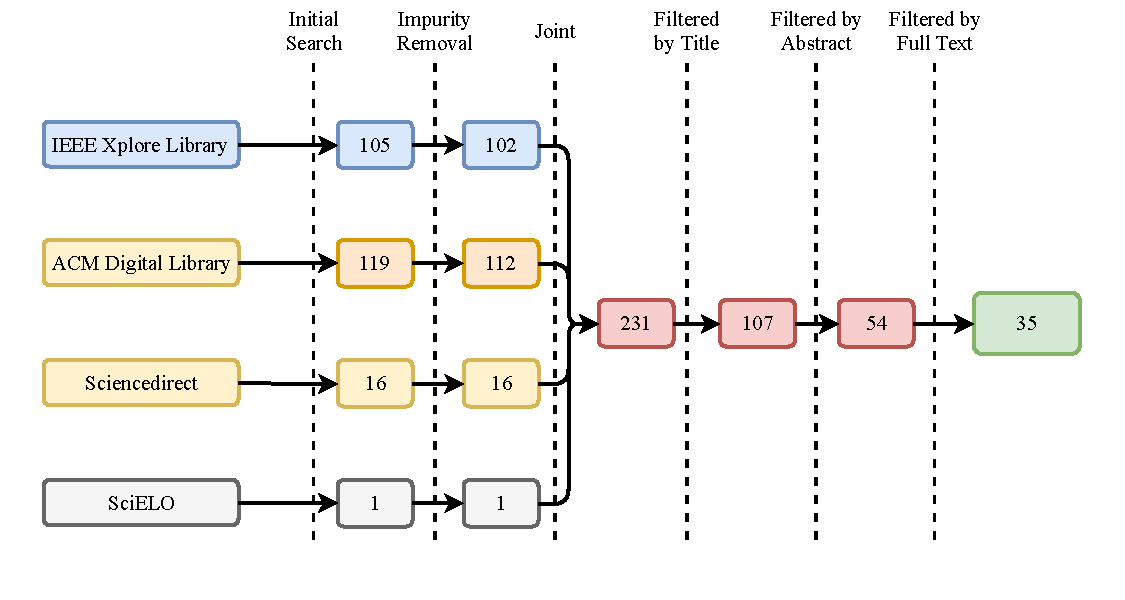
\includegraphics[scale=0.7]{Images/Article_selection.pdf}
\caption{Systematic mapping study - article selection.}
\label{article_selection}
\end{figure*}

We found 241 articles in the initial search before applying the exclusion criteria. After that, we performed the impurity removal that removes 10 (4.15\%) articles. Then, we joint the articles resulting in 231 articles. So, we filtered by title resulting in 107 (46.32\%) articles. Continuing the process, we perform a filter in abstract resulting in 54 (50.47\%) articles. Finally, we apply the exclusions criterion in the full text remained 35 (64.81\%) articles. These articles are the baseline for the study. Table~\ref{table_articles} shows an overview of all primary studies with the identifier, reference, publication year, publisher, and type.

\begin{figure*}[h!bt]
\centering
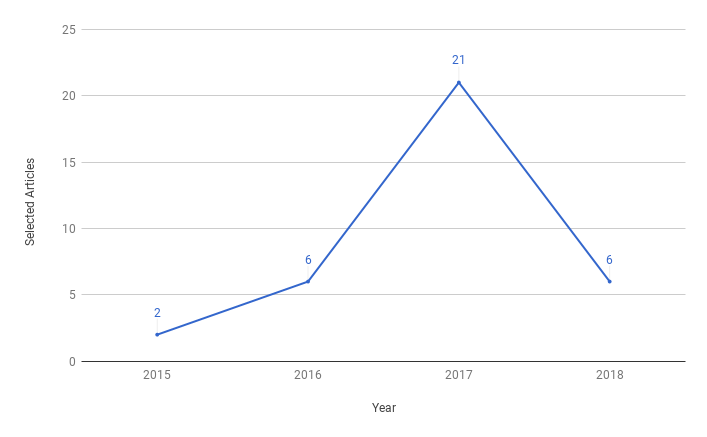
\includegraphics[scale=0.5]{Images/publication_chronology.png}
\caption{Publication chronology.}
\label{chronology}
\end{figure*}

In Figure~\ref{chronology}, we present the evolution of the selected publications over the years, covering from 2015 to 2018. This figure shows that we find recent articles in our research demonstrating that microservice is a new trend.

\begin{figure*}[htb]
\centering
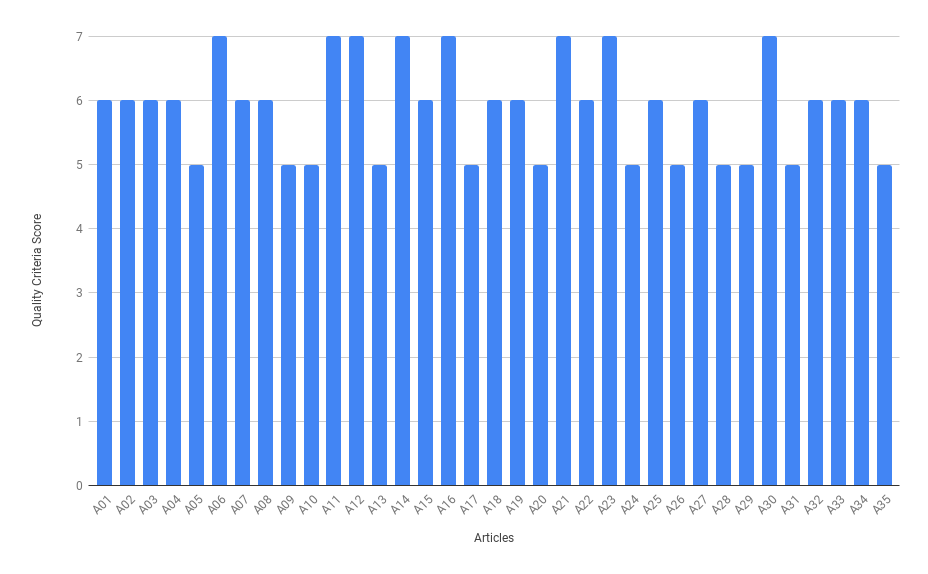
\includegraphics[scale=0.40]{Images/Quality_chart.png}
\caption{Quality assessment of the articles.}
\label{quality_chart}
\end{figure*}

\subsection{Performing the Quality Assessment}
In Figure~\ref{quality_chart}, we show the quality criteria score of the articles based on the quality assessment criteria proposed in Table~\ref{table_questions}. The quality criteria score for each article obtained is shown on the vertical axis and the studies themselves on the horizontal axis, from 1 to 35. This figure demonstrated that the articles responded positively to at least 5 out of 7 quality assessment criteria. For instance, several articles do not comment on or cite possible future studies in general because they are conclusive articles, with a conclusion on its assessment. Besides, some articles do not address the literature review, background, or context, because they are technical articles.

\subsection{Answers to the Research Questions}

Finally, to address the general and specific research questions, we have identified the following.

\subsubsection{CG1 How would the microservice performance and scalability appear?}
\begin{table*}[!bt]
\centering
\renewcommand{\arraystretch}{1.5}
\caption{Properties of microservice performance and scalability in articles.}
\label{table_CG1}
\begin{tabular}{ll@{\hspace{8em}}l}
\hline
\multicolumn{2}{l}{Group and item} & Description \\ \hline

\multicolumn{2}{l}{\textbf{Evaluation}} &  \\
 & Metrics & Metrics used to evaluate the performance and scalability (see subsection SQ1) \\
 & Algorithm & Algorithms to evaluate performance and scalability (see subsection SQ1) \\
 
\multicolumn{2}{l}{\textbf{User Application}} &  \\
 & Application classes & Application types of microservices (see subsection SQ2) \\
 
\multicolumn{2}{l}{\textbf{Architectures}} &  \\
 & Distributed system & Describes the main architecture models (see subsection SQ3) \\
 & Virtualization & Describes the virtualization type of microservices (see subsection SQ3) \\
 
\multicolumn{2}{l}{\textbf{Communication}} &  \\
 & Patterns & Communication patterns of microservices (see subsection SQ4) \\
 & Protocol & Communication protocol of microservices (see subsection SQ4) \\ \hline
\end{tabular}
\end{table*}
We search characteristics of microservice performance and scalability in articles. We want to find metrics, patterns, protocols, architecture and applications classes of microservice. We review the selected articles to find these characteristics. Table~\ref{table_CG1} presents the results for this review. This table leads the remains research questions.

We used this classification to build the taxonomy (present in section taxonomy). We believe that this taxonomy could help to classify, compare, and evaluate different architectures and solutions for microservices. Table~\ref{table_CG1} presents four groups: (1) Evaluation, (2) User Application, (3) Architectures, and (4) Communication. Each item from the table has a brief description of the classification. Furthermore, the items have a binding with the specific research question that explores the item.

\subsubsection{CG2 What are the motivations for analyzing and improving microservice?}
\begin{table*}[tb]
\centering
\renewcommand{\arraystretch}{1.5}
\caption{Motivations to analyze and improve microservice.}
\label{table_CG2}
\begin{tabular}{llll}
\hline
\multicolumn{2}{l}{Group and identifier} & Description & Reference articles \\ \hline

\multicolumn{2}{l}{\textbf{Metric analysis}} &  &  \\
 & Energy & Analysis of the energy consumption of microservices & A01, A04 \\
 & Cost & Evaluate the microservice application cost & A01, A03, A08, A09, A13, A15, A28 \\
 &  &  & A31 \\
 & Performance & Analysis of the microservice performance & A01, A03, A04, A05, A06, A07, A08, \\
 &  &  & A09, A10, A11, A12, A13, A14, A15, \\
 &  &  & A16, A17, A18, A19, A20, A21, A22, \\
 &  &  & A23, A24, A25, A26, A27, A29, A30, \\
 &  &  & A31, A32, A33, A34, A35 \\
 & Reliability & Analysis of the reliability of the microservice application & A04, A12, A17, A23, A26 \\
 
 \multicolumn{2}{l}{\textbf{Deployment}} &  &  \\
 & Update & Evaluate the impact of microservice update on performance & A15, A24, A31 \\
 
 \multicolumn{2}{l}{\textbf{Architecture}} &  &  \\
 & Communication & Analysis of the communication impact in performance & A06 \\
 & Scalability & Evaluate the scalability of the microservice architecture & A01, A02, A04, A05, A06, A07, A10 \\
 &  &  & A11, A18, A23, A25, A27, A28, A31 \\
 &  &  & A32 \\ \hline
\end{tabular}
\end{table*}
In this question, we want to find what are the motivations from the articles to analyze the microservice behavior. The major contribution of this question is presents the common concerns in microservice performance and scalability aspects. 

Table~\ref{table_CG2} presents the result from our research on this question. This table has three groups to describe the concerns in microservice related to metric analysis, deployment, and architecture. 
The metric analysis group aims to answer why is necessary to analyze metrics in a microservice environment, ranging from performance investigation to measure the reliability of the system. Besides that, another interest involves examination of microservice cost, particularly interesting in public clouds, and metrics to analyze the energy consumption.

The second group is the deployment that a investigate the impact of microservice update on the performance and scalability. With DevOps, programmers continually modify the microservice source-code, so it is difficult to know the right moment to deploy some modification.

Finally, the Architecture group analyze the concerns when a developer wants to create a microservice architecture, like how to guarantee the system scalability and how to implement the communication between microservices.

\subsubsection{SQ1 Which are the metrics and algorithms used to evaluate microservice?}
\begin{table*}[p]
\centering
\renewcommand{\arraystretch}{1.5}
\caption{Types and metrics used to evaluate microservice behavior.}
\label{table_SG1}
\begin{tabular}{llll}
\hline
\multicolumn{2}{l}{Group and identifier} & Description & Reference articles \\ \hline

\multicolumn{2}{l}{\textbf{Metrics}} &  &  \\
 & CPU & Percentage of CPU utilization & A02, A06, A08, A09, A13, A14, A16, \\
 &  &  & A17, A19, A20, A23, A24, A26, A30, \\
 &  &  & A32, A33 \\
 & Memory & Memory consumption & A06, A08, A16, A17, A20, A23, A33 \\
 & Execution time & Application execution time or response time & A01, A03, A04, A05, A07, A08, A10, \\
 &  &  & A12, A15, A19, A20, A24, A25, A28, \\
 &  &  & A29, A30, A31, A34 \\
 & Task queue & Length of task queue & A05, A20, A25, A26, A27 \\
 & Network throughput & The network throughput between the microservices & A06, A11, A16, A17, A18, A21,\\
 &  &  & A22, A23, A32 \\
 & Task processing rate & Number of tasks processed per time & A01, A10, A12, A20, A24, A30, \\
 &  &  & A31 \\
 
 \multicolumn{2}{l}{\textbf{Types}} &  &  \\
 & Relative & The share that each container has of the resources used & A01, A02, A03, A04, A05, A06, A07, \\
 &  &  & A08, A09, A10, A11, A12, A13, A14, \\
 &  &  & A15, A16, A17, A18, A20, A21, A22, \\
 &  &  & A23, A24, A25, A26, A27, A28, A29, \\
 &  &  & A30, A31, A32, A33, A34 \\
 & Absolute & Actual utilization of host system resources & A19 \\
 
\multicolumn{2}{l}{\textbf{Algorithm}} &  &  \\
 & Reactive & Perform decisions when reaches a threshold & A02, A05, A07, A09, A14, A19, A20, \\
 &  &  & A23, A24, A25, A26, A27, A33 \\
 & Proactive & Perform decisions proactively, before reach a threshold & A01, A12, A13, A16, A17 \\
 
\multicolumn{2}{l}{\textbf{Proactive algorithm}} &  &  \\
 & Pattern analysis & Analyze application patterns to improve performance & A01, A17 \\
 & Mathematical model & Use mathematical models to analyze the behavior & A12, A17 \\
 & Machine learning & Use machine learning to analyze the behavior & A13, A16 \\ \hline
\end{tabular}
\end{table*}
To answer this research question, we analyzed all selected studies that involved research of the metrics and algorithms used in microservice evaluation. Table~\ref{table_SG1} summarized the results of this analysis. We divided this table into four groups.

The first group presents the metrics found in the studies. We found both metrics of host health, like CPU and memory, and application status, like execution time and task queue.

Another group is the metrics types used to evaluate the application. We associated this group with metrics that show the host health such as CPU and memory. There are two types of metrics: (1) Relative metrics and (2) Absolute metrics. In Relative metrics, the value of a metric is just the portion that the host allocates to container/virtual machine. In Absolute metrics, the value is the actual utilization of host resources.

After dividing the metrics, we show the algorithms to evaluate these metrics and perform actions. We found two types of algorithms: (1) Reactive and (2) Proactive. In the reactive form, the system performs an action when a threshold reaches. Already in Proactive form, the system predicts an action before a threshold reaches.

Finally, the last group divides the Proactive form in the algorithms to predicts the application behavior. We found three types: (1) Pattern analysis which matches the application behavior to a template, (2) Mathematical model which applies some mathematical model to analyze the application behavior and predicts future values, and (3) Machine learning which uses a machine learning, such as neural network, to predicts system behavior.

\subsubsection{SQ2 Which are microservice applications classes?}
\begin{table*}[tb]
\centering
\renewcommand{\arraystretch}{1.8}
\caption{Microservices applications types.}
\label{table_SG2}
\begin{tabular}{l@{\hspace{1em}}l@{\hspace{3em}}l@{\hspace{2em}}l}
\hline
\multicolumn{2}{l}{Group and identifier} & Description & Reference articles \\ \hline

\multicolumn{2}{l}{\textbf{Transactional}} &  &  \\
 & Web requests & Requests to a host, like HTTP requests & A01, A07, A11, A14, A15, A16 A24, \\
 &  &  & A25, A27, A30, A31, A33 \\
 & Streaming & Multimedia streaming, like audio/vídeo & A13, A17 \\
 & Data transfer & Data transfer of files & A02, A28 \\
 
\multicolumn{2}{l}{\textbf{Batch}} &  &  \\
 & Image Processing & Processing to transform a image & A03, A34 \\
 & Mathematical model & Computation to resolve a mathematical problem & A08, A09, A19, A32 \\
 & ERP & Enterprise Resource Planning & A10 \\
\multicolumn{2}{l}{\textbf{IoT}} & Internet of things & A23, A26 \\ \hline
\end{tabular}
\end{table*}
Now, we want to know what are the classes of the microservice application that articles used. It is crucial because each class has a different approach to evaluate and improve application performance and scalability. For example, transactional applications have a long execution time compared with a batch application. So the best algorithm to use in this type of application is different. 

Table~\ref{table_SG2} shows the classes of the application that we found in our review. We divided the application class into three main groups. The first one is the Transactional application, such as web requests, data transfer, and streaming. This type of application needs to resolve many requests to a server. 

Another type of application is the batch applications that involves image processing, mathematical model, and enterprise resource planning. Unlike the transactional application, the batch application has one request and perform processing.

The last group of application is the Internet of things applications. This class of application involves sensors that produce data. A microservice application can process the data generated by sensors to provide some useful information.

\subsubsection{SQ3 What are the distributed system architecture of microservice applications?}
\begin{table*}[tb]
\centering
\renewcommand{\arraystretch}{1.8}
\caption{Distributed system architecture of microservice applications to improve performance and scalability.}
\label{table_SG3}
\begin{tabular}{llll}
\hline
\multicolumn{2}{l}{Group and identifier} & Description & Reference articles \\ \hline

\multicolumn{2}{l}{\textbf{Architecture}} &  &  \\
 & Cache based & Use a cache to improve microservices performance. & A03, A25, A29, \\
 & Load balancer & A load balancer defines the better host to perform tasks. & A05, A06, A15, A20, A22, A24, A31 \\
 &  &  & A34 \\
 & Mobile agent & A agent migrates to each host to evaluate and adjust the system. & A35 \\
 & Cloud & Elasticity feature to improve performance. & A01, A02, A05, A07, A09, A12, A13, \\
 &  &  & A14, A17, A19, A20, A23, A24, A25, \\
 &  &  & A27, A28, A33 \\
 
\multicolumn{2}{l}{\textbf{Elasticity}} &  &  \\
 & Vertical & Increases/decreases machines/containers capacity. & A33 \\
 & Horizontal & Add and remove computer nodes. & A01, A02, A05, A07, A09, A12, A13, \\
 &  &  & A14, A17, A19, A20, A23, A24, A25, \\
 &  &  & A27, A28 \\
 
\multicolumn{2}{l}{\textbf{Virtualization}} &  &  \\
 & Virtual machines & Operating system and hardware virtualization. & A01, A05, A08, A09,  A22, A23, A24, \\
 &  &  & A30, A32, A35 \\
 & Containers & Operating system virtualization. & A02, A03, A08, A11, A14, A16, A17, \\
 &  &  & A18, A19, A21, A24, A25, A27, A28, \\
 &  &  & A30, A31, A32, A33 \\ \hline
\end{tabular}
\end{table*}
Another result was the identification of distributed system architecture used in microservice applications. The definition of a distributed system is important to improving scalability and performance. Table~\ref{table_SG3} presents these results. 

We found three types of information. The first group is the architecture used in each article. We found four architectures: (1) Cache based that involves a cache of microservices or cache of response, (2) Load balancer that defines the best host to process the requisitions, (3) Mobile agents that involve an agent that migrate between hosts and adjust the host, and (4) Cloud that we detailed in section~\ref{background}.

The second group detail how the cloud could improve performance and scalability using elasticity. Elasticity could be vertical or horizontal. We explain this in section~\ref{background}.

Finally, the last group is the virtualization to cloud computing. We divided into (1) Virtual machines and (2) Containers. We detailed this in section~\ref{background} too.

\subsubsection{SQ4 Which are communication patterns and protocols to microservice?}
\begin{table*}[tb]
\centering
\renewcommand{\arraystretch}{1.8}
\caption{Communication patterns and protocols to microservice.}
\label{table_SG4}
\begin{tabular}{llll}
\hline
\multicolumn{2}{l}{Group and identifier} & Description & Reference articles \\ \hline

\multicolumn{2}{l}{\textbf{Patterns}} &  &  \\
 & Direct & The microservices communicates directly. & A13, A17, A22, A24, A28, A30 \\
 & Gateway & Use a gateway between the microservices. & A02, A06, A11, A15, A19, A20, A29, \\
 &  &  & A31, A34 \\
 & Message BUS & Use a message BUS to communicates between microservices. &  A06, A27, A34 \\
 
\multicolumn{2}{l}{\textbf{Protocol}} &  &  \\
 & HTPP/REST & Use REST API to communicates with microservices. & A02, A04, A05, A06, A08, A09, A14,  \\
 &  &  & A16, A24, A28, A31, A33, A35 \\
 & AMQP & Application layer protocol for message-oriented middleware. & A27, A34 \\
 & RPC & Remote protocol call. & A22, A29 \\ \hline
\end{tabular}
\end{table*}
The last question involves determinating the communication patterns and protocols to deploy microservice applications. Table~\ref{table_SG4} detailed the results found.

First, we classified the communication patterns of microservice using the three types explained in section~\ref{background}: (1) Direct communication, (2) Gateway communication, and (3) Message BUS communication.

So, we divided the articles into protocols used in communication between microservices and external applications. We found three types of protocol: (1) HTTP requests using REST API, (2) AMQP protocol that implements a queue of tasks, and (3) Remote protocol call. 


%=======================================================================
% Taxonomia
%=======================================================================
\section{Taxonomy Proposal}
\label{Taxonomy-proposal}
In this section, we will discuss the results found in our research. First, we present a taxonomy that we created using the results from section~\ref{results}. This taxonomy can be useful to classify solutions of microservice performance and scalability.

After that, we perform a discussion about the results found in the reviewed articles. This discussion aims to presents what are the more often use to improve and analyze microservice applications related to scalability and performance. Finally, we show some tendencies in microservice implementations. 

\subsection{Taxonomy}
\begin{figure*}[htb]
\centering
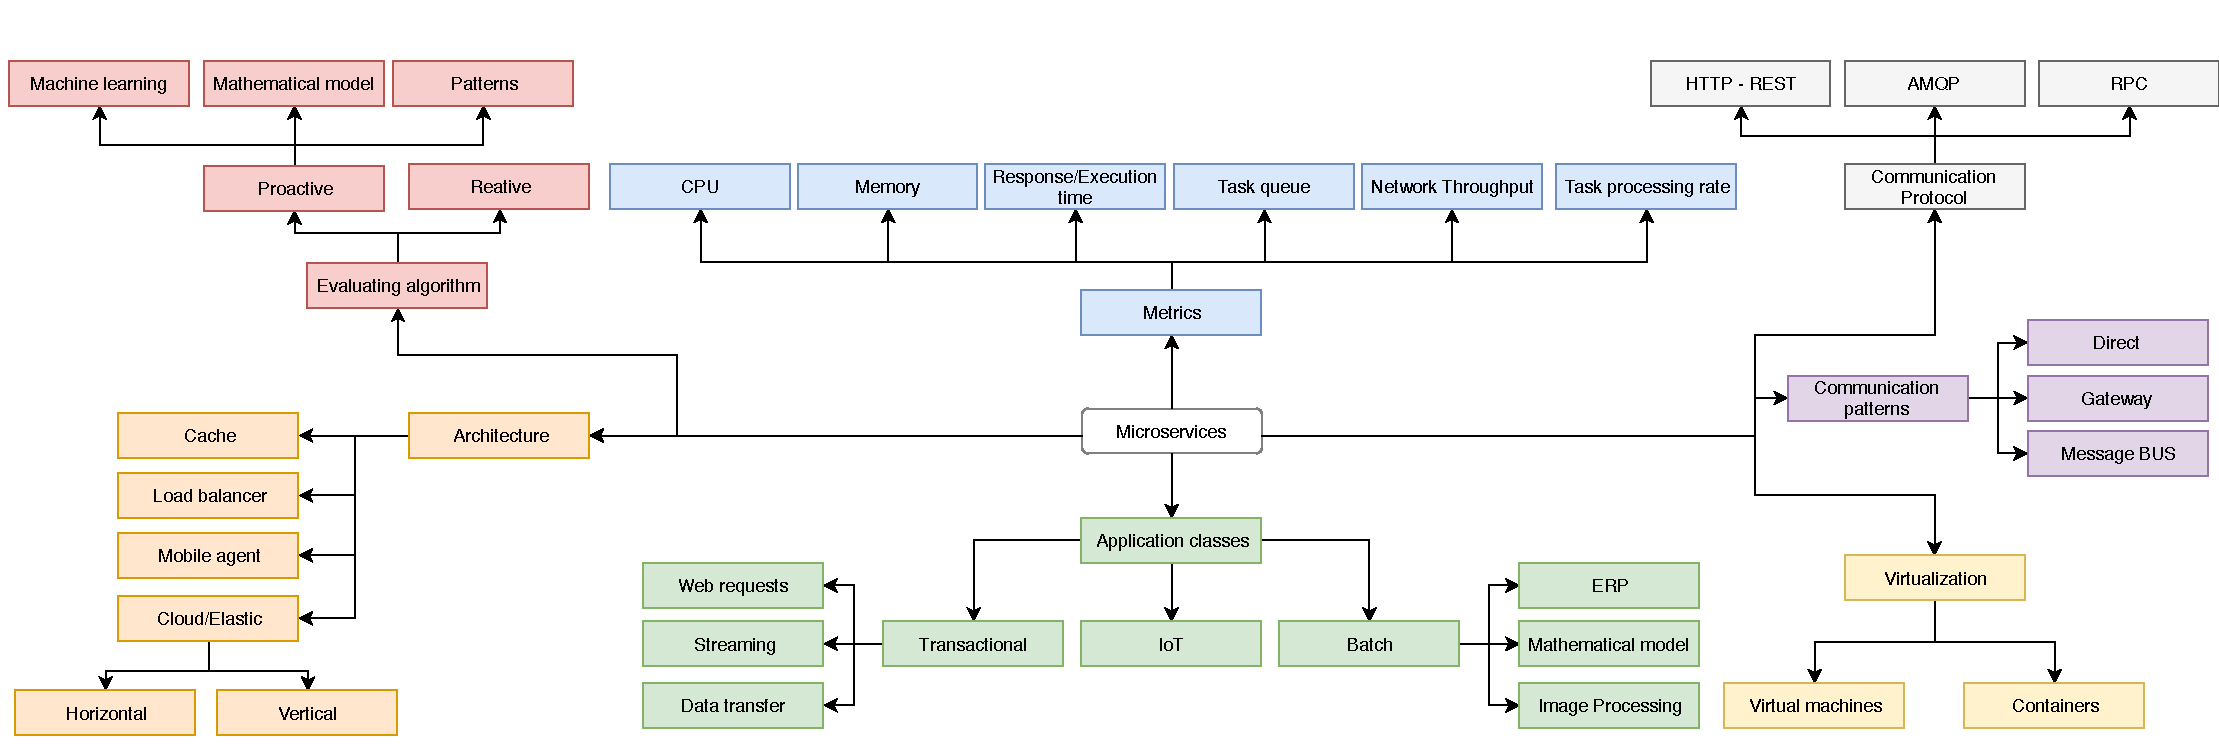
\includegraphics[scale=0.50]{Images/Taxonomy.pdf}
\caption{Microservice scalability and performance taxonomy. We divided into seven main groups: (a) Application classes, (b) Metrics, (c) Architecture, (d) Evaluating algorithm,  (e) Communication Protocol, (f) Communication Patterns, and (g) Virtualization.}
\label{taxonomy-figure}
\end{figure*}

Analyzing the results from the section~\ref{results}, we present the performance/scalability taxonomy from figure~\ref{taxonomy-figure}. In this section, we will present the classification, and in the next section, we will show how this classification appears in reviewed articles. We used seven main groups to describe how and when improvements in microservice performance and scalability appear. 

\subsubsection{Application classes}
First, we defined the application class of the microservice. It is essential to define the class of application because each class has a well determinate behavior and requirements. In the discussion, we will use this classification to related with the others research questions. We found in the reviewed articles three application classes main groups: (a) Internet of Things, (b) Transactional, and (c) Batch.

The Internet of Things (IoT) application class consists of applications with integration to sensors. A well-accepted architecture for IoT is EPCglobal~\cite{ArmenioJohnson2009The1.3}, and we will use to exemplifies microservice in IoT. This architecture has three main components: RFID readers, Application Level Events (ALE), and EPC Information Services (EPCIS). The RFID readers are the hardware layer that contains the sensors. The Application Level Events (ALE) is responsible for filtering and consolidate the sensor information. The last component is the EPC information service (EPCIS) that provides a service to access the data of readers. Microservice appears in ALE and EPCIS components. For example, EPCIS needs to scalable according to application requests.

The second application class is the transactional applications. Applications of this class usually have many application requests over the internet. We found three applications types in this class: Web Requests, Streaming, and Data Transfer. In Web Requests, the users request an internet address. The application performance is directly related to the amount of users requests. In a moment of the day, the system could have more requests than in others. In Streaming applications, the user receives many multimedia data. If the application lost some packages, the quality is not affected. Finally, the last transaction application is data transfer. In this type of application, the user requests some file and download this data from the server. Another application example is transfer files between two hosts.

The last application class is the batch applications. In this application class, the user executes one solicitation, and wait for the application ends. The application executes the data processing, that can take time. This application class is typically the class application used in high performance. We found three types of this class: Enterprise Resource Planning (ERP), Mathematical Model, and Image Processing. Enterprise Resource Planning (ERP) is the application to resolve some business issues. One example of ERP is ERP Payroll that needs to calculate the value to pay to the employees. The Mathematical Model try to resolve some not trivial mathematical problems. Some problems take some time to finalize. To finalize the problem in time, we can divide the problem in multiples microservices. Image processing application is applications that apply a change in some image. This application needs to apply a change in every image pixel, and this takes some time. Like the Mathematical Model, we can divide this problem in some microservices.

\subsubsection{Metrics}
Secondly, we classified the solutions by the metrics used in its analysis. This classification is essential to what metrics evaluate in applications. We found six metrics: (a) CPU, (b) Memory, (c) Response/Execution time, (d) Task queue, (e) Network Throughput, and (f) Task Throughput. The (a), (b), and (e) are metrics that can be measured directly in a host, while the others metrics are application metrics that needs some code instrumentation to be measured.

The first metric is the CPU that indicates the usage percentage from the Central Processing Unit. Usually, this metric shows system performance and the sum of work handled by the host. We will demonstrate in the discussion that this metric is widely used to analyze the performance.

Another widely used metric is memory utilization. This metric shows how much the application is retrieving data from physical to virtual memory and vice-versa. This paging can affect the performance because the CPU needs to stop the processing to manage the memory.

The Response/Execution time describes the metric how long the application or microservice takes to respond or finalize the processing. This metric directly indicates the microservice performance. For example, a microservice usually takes 5 minutes to finalize. At any time, this time grows to 10 minutes, so the microservice needs more resources.

The fourth metric is the task queue. Every microservice has a requisition queue that contains all microservice requisitions. An analyze in how this queue grows it is an essential metric to know how to adjust the microservice.

Another metric is the Network Throughput that shows the communication throughput in a system. According to an application grows, the microservice grows and have more communication. So, the Network Throughput affects the whole application performance.

The last metric is the task processing rate. This metric shows the number of jobs processed per time. For example, this can indicate that a microservice process five jobs per second. This metric directly shows the microservice performance.

\subsubsection{Architecture}
The third group is the architecture used to improve the microservice application. In this group, we found four architecture. 

The first is the cache based architecture that improves the microservice using a cache to avoid reprocessing the requests. This architecture is particularly useful in database microservices that perform a lot read actions. 

The second architecture is the load balancer. This architecture implements a load balancer that finds the better microservice node to process the incoming request. We found two ways to determine the better node to process a request: (a) On the fly decision and (b) define each node computation capacity. In (a) the load balancer defines on the fly which node will compute the incoming request based on the current workload of each node of the microservice application. This way is not an easy task to do on the fly and can affect the application performance. In (b) the system evaluates the computation capacity of each node. The system sends a simple request to each node and saves a node metric (e.g. response time). The load balancer used this metric to make a decision.

The third architecture is the mobile agent. This architecture involves an agent that migrates to the hosts. The agent migrates to a host to evaluate the current state of this host and to make adjustments aiming to improve the host performance.

Finally, the last architecture is the cloud. The previous architecture can use the cloud but does not use the high cloud differential: elasticity. For this reason, we created this group. When we discuss the reviewed articles, we will present how vital is elasticity to microservice, because of the cloud using elasticity is the most used architecture for microservice. Elasticity has two methods: (a) Horizontal and (b) Vertical.  In (a) the cloud adds or removes nodes and in (b) the cloud increases or decreases nodes resources. We described the elasticity in section~\ref{background} already.

\subsubsection{Evaluating algorithm}
The next group is the evaluating algorithm. This group describes how the system evaluates the metrics to perform actions. First, we divided into two algorithms: (a) Reactive and (b) Proactive. 

In (a) the system reacts to a change or collects metrics when a threshold reaches. For example, the system performs an action when the CPU of a node reaches 80\%. The reactive form has an easier implementation than the proactive, but this form can impact in the application performance. Could be too late for the application act just when a threshold reaches. Besides that, the application can be in an invalid state for a while. 

In (b) the system predicts when acting. Differently from reactive form, in the proactive form, the system collects metrics and predicts before an invalid state reaches. This algorithm is not too easy to implements, comparing to the reactive form. We found three proactive algorithms: Machine Learning, Mathematical Model, and Pattern Analysis. 
In the first proactive form, the system uses a machine learning algorithm, e.g. Support Vector Regression and Neural Networks, to predict metrics. Usually, machine learning algorithms need a period to learn before starting to predict. This requirement is a drawback of this approach.

Another proactive algorithm is the Mathematical Model. In this approach, the system uses an algorithm, such as Autoregressive Moving Average (ARMA) and Autoregressive Integrated Moving Average (ARIMA), to predict metrics. While machine learning needs a reasonable period for learning, Mathematical models start to predict as soon as possible. However, mathematical models have a less accurate output and minor outlier tolerance. 

The last proactive algorithm is the Patterns Analysis. In this approach, the system tries to match the current state of the application with to some defined pattern. If the match occurs, the system act. This approach is one of the most challenging algorithms to apply in a system to evaluate performance and scalability to microservices, comparing with machine learning and the mathematical model. Real applications can have values variations that the analysis need consider.

\subsubsection{Communication Protocol}
According the application grows, the quantity of microservice grows, and them needs to communicate with each other. So, the communication protocol affects the microservice performance. We found three protocols: (a) HTTP - Rest, (b) AMQP, and (c) RPC. 

The first protocol is the HTTP - Rest. This protocol provides interoperability between internet system. Usually, the microservices implement web service Restful. The second protocol is AMQP (Advanced Message Queuing Protocol) that implements a queue message protocol. Finally, the last protocol is the RPC (Remote Procedure Call). This protocol allows a procedure to execute in a different address space. 

\subsubsection{Communication Patterns}
As explained in the background section, there are three microservice communication patterns: (a) Direct, (b) Gateway, and (c) Message BUS.

In the Direct Communication, the microservices communicate between themselves directly and without any layer between the components. This pattern has a simpler implementation comparing with others patterns.

The second pattern is the Gateway. In this implementation, each microservice has a gateway that translates the different communication protocols. Besides that, this gateway can router when a microservice has some replicas.

The last pattern is the Message BUS. This pattern has a Message BUS that centralizes all requests to microservices. This Message BUS is a native router implementation because the first node to finalize takes another task from Message BUS.  

\subsubsection{Virtualization}
The last classification is the virtualization. This classification shows the virtualization level used in the microservice application. We found two virtualizations: (a) Virtual Machines and (b) Containers.

Virtual Machines (VMs) was the main virtualization type until recently. VMs are virtualization of a computer environment that allows the same functions that a real computer. A VM is isolated from the computer host. A node can host such VMs as its resources allow.

Such as VMs, Containers are an isolated and virtual computer environment. While each VM runs an entire operating system, each operating system runs several Containers. Containers are more lightweight than VMs.

%=======================================================================
% Desafios
%=======================================================================
\section{Discussion}
\label{Discussion}
In this section, we will discuss the reviewed articles. Our objective is to explore what is state of the art regarding microservice performance and scalability. First, we will investigate question by question showing the items with higher usage. After that, we will cross-reference the items showing some trends. 

\subsection{CG1 How would the microservice performance and scalability appear?}
This question guides our remains research questions and our taxonomy that we presented in the previous section. Table~\ref{table_CG1} shows the result of this question. We divided into four main groups. We analyze each group in the following sections.

The first group is the Microservice Evaluation, one of the most important contributions of this survey. With this group, we want to describe the metrics and algorithms to evaluate the microservices. This group helps to classify the solutions for microservice.

The second group is the microservice application type. This group is essential because this shows us the microservice application trends. Determining the application type, allow us to indicates the better approach in performance terms and scalability.

The third group describes the microservice architectures found in reviewed articles. This group demonstrated how the performance and scalability appear in the architecture. 

The last group presents communication patterns and protocols. Communication is a crucial element in microservice since a microservice collection build an application. So, each microservice needs to communicate with the others to compose an entire application.

\subsection{CG2 What are the motivations for analyzing and improving microservice?}

Now, we want to determine the primary motivation for the reviewed articles for analyzing microservice metrics. It is crucial to define the motivation to relate this to the design decisions. 

Table~\ref{table_CG2} demonstrated the results from this question. We will analyze the three groups together because there is not a real division in this question. We divided this just for better comprehension in previous sections. 

The primary concern, about analyzing microservice metrics, is the evaluation of microservice performance. Our results show that 94.2\% of total articles indicate this concern. This concern implies analyzing the application response time, how long the application takes to finalize a job, how much jobs the application process in a second, and others motivations related to execution.

The second concern is the scalability, with 42.85\% of articles. Scalability is an essential motivation to analysis the microservice. Application requests may increase, and the architecture needs to deal with this increase. 

Another motivation is to evaluate the cost of the application. This concern is particularly important when using a public cloud because the cloud provider charges the user for the utilization. In our research, 22.86\% of the articles present this motivation. 

The reliability is another motivation to evaluate microservices. This motivation involves ensuring that the microservice responds correctly and without fail.  We found this motivation in 14.29\% of total articles.

The microservice update impact is another concern that we found in 8.57\% of total articles. This update can impact in microservice because the microservices needs change on the fly without stopping the application. 

The remain motivations for analyzing microservice are energy consumption and communication. Energy consumption appears in 5.71\% of total articles and Communication in 2.86\%. While the first one analyzes the impact of microservice on energy consumption, the Communication evaluates the impact of the communication between microservices in the application.

The above results show that the primary motivation to evaluate and analyze microservice metrics is to know the application performance and scalability. Regarding performance, a monolithic application has a better performance than the microservice approach. One motivation for the better performance in the monolithic approach is the communication between microservices. This evaluation is essential to keep performance after migration from monolithic to microservice. Also, the application needs to handle the increase in user requests, so evaluate scalability is another important motivation. 

When the microservice application is in a public cloud provider, the cost evaluation of the application is an important motivation. The resource management is crucial to submit a microservice to cloud, and this management needs to avoid resources wasting. Maintain an unnecessary resource online is a waste of money in a public cloud.

\subsection{SQ1 Which are the metrics and algorithms used to evaluate microservice?}

In this section, we will describe the metrics and algorithms used to evaluate microservice that we found in reviewed articles. Table~\ref{table_SG1} shows the result of this question. First, we will present the most utilized metrics. After that, we describe the metric types found. Finally, we show the algorithms to analyze these metrics.

The primary metric used in microservice evaluation is the execution time. This metric appears in 51.43\% of total articles. Analyze execution/response time is vital because this metric shows a direct relation with application performance. It is a useful performance metric because this indicates how long the microservice takes to answer. The system can compare the desired time with the time measured to make decisions.

Another metric used in microservice evaluation is the CPU. We found this metric in 45.71\% of total articles. Unlike the execution time, the manager can measure CPU directly from application host. While the execution time needs instrumentation to be measured, the CPU shows the state of the microservice host without instrumentation. If the microservice host has a high CPU percentage, this affects the host performance and indicates that this host has a high workload to process.

The third metric is the network throughput, which appears in 25.71\% of total articles. This metric presents the communication throughput between the microservices and between the user and the application. Like CPU, some host managers provide this metric directly. Network throughput affects the performance. A low throughput impacts the communication between the microservices, so a microservice needs wait for all data before starting the processing.

With 20\% of total articles, the next metric is the task processing rate. This metric indicates the number of tasks processed per time (e.g. 20 jobs/s). Like execution time, task processing rate needs instrumentation to be measured. Also, this metric is a useful performance metric because this indicates how many tasks the microservice can process in a period. With this rate, the manager can analyze requests patterns and make adjustments in the host.

Also with 20\% of total articles, another metric is the memory. This metric affects the performance when the virtual memory is full, and the system needs to wait a time for retrieving data from physical to virtual memory. If the host has low memory, this frequently occurs. 

The last metric, with 14.26\% of total articles, is the task queue. This metric shows how long is the microservice task queue. If a microservice has many requests for processing and the task processing rate is not good enough, this microservice queue will grow and, consequently, the response time will increase. 

After we presented the metrics found in the reviewed articles, we will describe the metrics types. We found two types: (a) Relative and (b) Absolute. The relative metric type demonstrates the share of CPU used by one container concerning other containers. For example, if a host has two containers and each container use all allocated CPU, the measured value of each container will be 50\%. In absolute metrics, the measure values demonstrated the value of the container just concerning itself. In the same previous example, each container measured will show 100\%. Just one reviewed article detailed absolute metric~\cite{Casalicchio2017}, but many articles use one microservice in one container, so, in this case, the absolute and relative metrics have the same value.

Finally, we will describe the algorithms to evaluate the metrics that we found in reviewed articles. We categorized the algorithms in (a) reactive and (b) proactive. In the reactive approach, the system decides to act when a threshold reaches. This approach has a more straightforward implementation comparing with the proactive approach. The easier implementation can explain that we found more reactive approaches than proactive. We found 37.14\% of total articles to the reactive approach. The proactive algorithm tries to predict future behavior and perform an action before an undesirable state reaches. In the reviewed articles, 14.29\% use the proactive form. To predict future behaviors, we found three proactive classes: (a) Pattern Analysis, (b) Mathematical model, and (c) Machine learning. 

All three algorithms have the same percentage (5.71\%) of the total reviewed articles. In Pattern Analysis, the manager tries to match the actual behavior of the application with a pattern. Using this information, the manager can predict how the system will behave. Already in the Mathematical model, the manager uses one or many mathematical models to describe the application behavior. With this model, the predictor can extrapolate the values of the model to calculate future values. Finally, the last proactive class is machine learning. In this approach, the manager uses some algorithm, like a neural network, to define the system behavior. After train the algorithm, the system can simulate some cases to evaluate how the system will work. 

\subsection{SQ2 Which are microservice applications classes?}
In this section, we will describe the classes of the microservice application found in reviewed articles. With this classification, we can correlate the application classes with other questions. First, we divided into three groups: Transactional, Batch, and IoT. 

The transactional is the application class that involves many user requests over the internet. In this classes, we found three applications types: (a) Web requests, (b) Streaming, and (c) Data transfer. 

In (a), we have many user requests to a host, like a website. We found 34.26\% of total articles that address this application type. In (b) the application maintains a connection with the user to streaming multimedia data. We found 5.71\% of total articles to the streaming application type. Like the Streaming application type, the (c) also has 5.71\% of total articles. This application class describes an application that transfer data between servers and users.

The second group is the batch application type. This group involves applications that the user executes one solicitation and wait for the application ends. We found three application types into this group: (a) Mathematical, (b) Image processing, and (c) ERP. 

In (a), the user needs to process a mathematical problem. This problem can take some time to finalize, so the user needs to wait for the end. We found 11.43\% of total articles in this class. In the application type (b), the user needs to manipulate some image, like add saturation. To this type, we found 5.71\% of total articles. Finally, in the (c), the user has many functions to his enterprise. The user executes one function and waits for the end. We found 2.86\% of total articles in this type.

The last group is Internet of Things. This application class consists of applications with integration to sensors. We found  5.71\% of total articles in this application class.

\subsection{SQ3 What are the distributed system architecture of microservice applications?}

Now, we will describe the distributed system architecture of microservice applications. First, we will describe the architectures. We have four architectures: Cloud, Load balancer, Cache Based, and Mobile agent.

The first architecture is the cloud. We found 48.57\% of total articles that use the cloud to improve the microservice application. This result does not mean that the others architectures do not use the cloud but means that these articles use as the primary architecture of the cloud.

The second architecture is the load balancer. In this architecture, the system has a component named as the load balancer. This component directs the requisitions to the right node to process. In our review, 22.86\% of articles use a load balancer.

The next architecture is the cache based. This architecture consists of a component that evaluates the requisition. If the answer for this requisition is in the cache, retrieve the cached answer. 8.57\% of articles use cache architecture.

The last architecture is the mobile agent that we found 2.86\% in our review. Mobile agents consist of a component that migrates into each node and performs some action or measurement. 

Microservice applications widely use the cloud, as shown previously. One motivation to use the cloud is because of the elasticity. So, it is crucial to define the elasticity types found in the reviewed articles. We found two elasticity types: Horizontal and Vertical. 

In cloud computing, horizontal elasticity is the most used. We found 17 articles that use cloud computing as the primary architecture. Of these 17 articles, 16 articles implement horizontal elasticity. Horizontal elasticity is the ability to add and remove nodes on-the-fly. 

The vertical elasticity has few implementations. We found just one article that addresses vertical elasticity. In vertical elasticity, the system adjusts a node adding and removing resources, like CPU and memory. Previously the vertical need to stop the application. The most recent cloud providers indicate that is not needed to stop the execution anymore.

Another classification is the virtualization type. We found two types: Container and Virtual Machines. Containers are not a new concept but grow with the rise of Docker. We found 51.43\% of articles that use containers. This percentage demonstrate how the containers utilization surpassed the virtual machines utilization. 

We found 28.57\% of articles that use virtual machines yet. This percentage tends to decrease since the microservice is a perfect implementation for containers. The major difference between virtual machines and containers is that the container is virtualization at the operating system level. Already in the virtual machine, the whole system is virtualized, inclusive the operating system. So, the container has a minor boot start time comparing with the virtual machine.

\subsection{SQ4 Which are communication patterns and protocols to microservice?}
Finally, the last question is about communication. When a system migrates to microservice from monolithic, the first concern is the impact of communication in performance and scalability. Before microservice, the communication between the functions are in the same computer node, so this communication is not a factor to consider. With microservice, communication usually uses the internet, and the internet has a high impact on performance.

Finally, the last question is about communication. When a system migrates to microservice from monolithic, the first concern is the impact of communication in performance and scalability. Before microservice, the communication between the functions are in the same computer node, so this communication is not a factor to consider. With microservice, the communication usually uses the internet, and the internet has a high impact on performance. To analyze the communication, we divide this question into two groups: Communication patterns and Communication protocol.

The first is the pattern used to define all communication between microservices. We found three communication patterns: Gateway, Direct, and Message BUS. We detailed in the background section these three patterns.

The most used communication pattern is the gateway. We found 25.71\% of reviewed articles use the gateway communication pattern. One microservice characteristic is the programming language heterogeneity, that is each microservice could use a different language. So, this gateway is useful because the gateway translates the protocol between microservices.

In the direct communication pattern, the microservices communicate with each other directly.  Differently from the gateway, in this pattern, the programmer needs implements the same communication protocol in the different languages of each microservice. We found 14.29\% of articles that use this communication pattern.

The last pattern is the message BUS. In this pattern, the system uses a message BUS to communicate between microservices. So, the microservices get a task from the message BUS, process this task and return the result to message BUS. This result can be a task for another microservice. We found 8.54\% articles that use message BUS.

After describing the communications patterns, we will detail the communication protocols. We found three protocols: REST HTTP, AMQP, and RPC. The most used protocol is the REST HTTP. This protocol provides interoperability between internet system using web services. Usually, this protocol provides four operations: GET, POST, PUT, and DELETE. We found 37.14\% articles that use REST protocol. 

The two remains protocols are AMQP and RPC that we found 5.71\% articles. The Advanced Message Queuing Protocol (AMQP) is an implementation of a queue of messages. Finally, the last protocol is the RPC (Remote Procedure Call). This protocol allows a procedure to execute in a different address space.

\subsection{Tendencies}
Now, we will describe some tendencies to microservices. The previous section explains some tendencies analyzing each item of the research questions individually. In this section, we correlate the items, showing some trends to implement microservice analysis. We will explain this in three steps. First, we will correlate the motivations with the others research questions. After that, we will show the correlation of application type with others research questions. Lastly, we will describe other correlation found in the review.

\subsection{Motivation and Application type}
In this section, we will show the correlation found in our review between motivation and application type. All the four motivations that we will analyze in this section use the web requests application type. This result demonstrates the growth of web applications using microservices. Besides that, microservice is a structure for web applications, and this result confirms that.

The first motivation is the performance that we found 33 articles. In this motivation, we found 14 articles with performance motivation and transactional application type. Of these 14 articles, we found 12 articles that use a web requests application type. Evaluating the microservice performance of web applications is essential to improve the user experience. Differently from batch applications, in the transactional applications, the waiting time directly affects the application quality.

The scalability motivation appears in 15 of the reviewed articles. Like in performance motivation, the most used application type is transactional with 8 articles. Of these 8 articles, we found 6 articles that use a web requests application type. The scalability evaluation for web applications is especially necessary for web requests. In a web application, the number of users using the service affects directly the number of nodes necessary to maintain the server working properly. 

The third motivation is the microservice update that we found three articles. All three articles use web requests. The update motivation is a concern just in web applications since in this class the application the developer wants to update the application without stopping the user utilization. 

The last motivation is the cost motivation. We found eight articles with this motivation. Of these eight articles, three use web requests application type. Analyzing the cost of the web applications is essential especially when this application is in the cloud. 

\subsection{Motivation and Metrics}
Now, we will correlate the motivation with the metrics research question. The first motivation is performance. Of the 33 performance articles, we found 17 articles that use execution time. The execution time is a metric that directly indicates the application performance. With the execution time, the system can evaluate the performance of each microservice comparing the measured value with the expected value. This comparison determines the microservice state, and the manager uses to perform actions to improve performance (like adding more microservice nodes). 

Another metric used in performance motivation is CPU. We found 15 articles using the CPU as the metric to evaluate microservice. CPU indicates the usage percentage from the Central Processing Unit. For example, if a node has a high CPU percentage, this can indicate that this node has many tasks for processing. With this information, the system can add more resources to help this node in its job. 

Still in performance motivation, another tendency is the utilization of a reactive algorithm. We found 12 articles with the reactive algorithm. Applications use a reactive algorithm because this algorithm has a more natural implementation and does not need a learning period. Usually, the reactive algorithm has a lightweight implementation, in comparison with proactive algorithms. So, a more complex algorithm can impact the application performance.

The second motivation is scalability. Like the performance motivation, the scalability has as the primary metric of the execution time. We found eight scalability articles that use execution time. The execution time can indicate that a microservice is slower than expected. So, if the number of users increases and the microservice has a high execution time, the system delay to answer each user. Therefore, the manager needs to add more nodes. Like in performance motivation, another tendency in scalability motivation is the utilization of a reactive algorithm that we found six articles. The reactive utilization in scalability has the same motive that in performance motivation. 

The next motivation is the cost. The primary metric of this motivation is execution time, like the previous motivations. We found six articles that use execution time to evaluate cost. The relationship between cost and execution time is that the longer the execution time, the more costly is the application. Therefore, the execution time is the right metric to evaluate the cost of an application.

Finally, the last motivation is reliability. We found five articles that have reliability as motivation. Three of these five articles use CPU as the metric to evaluate the reliability. The CPU indicates the status of a node in a microservice environment. Therefore, if the system has many nodes with high CPU usage, possibly the application was in an undesirable state. Hence, the microservices starts to delay the answer or lost some packages. 

\subsection{Motivation and Distributed system}
The evaluation motivation guide the selection of the best microservice architecture. So, it is essential to define the correlation between the motivations and the distributed system in microservice applications. This section will present our results of this correlation.

Cloud computing appears as the most used architecture of four motivations: Performance, Reliability, Cost, and Scalability. This result shows that cloud computing is a tendency for microservice since these motivations are the primary motivations found. The performance and scalability evaluation of a cloud is an essential motivation because the cloud allows modifications on the fly in its environment to improve. Regarding cloud, we found 15 of 33 articles that have the motivation as performance and 8 of 15 that have the motivation as scalability.

The cost evaluation is essential in a cloud environment, mainly in a public cloud. In a public cloud, the client will pay for the time and resource usage. Therefore, the evaluation and improvement of the cost can be the success factor of a software. The cost evaluation combined with cloud computing appears in four of eight of reviewed articles about cost evaluation.

The four motivations that have cloud as the most used distributed system, also have the horizontal elasticity as the improvement policy. If a microservice environment has a node with much work to do, seems more useful to add another node to helps with the workload rather than add more resources in the node. It is not sure that increasing memory or CPU capacity will improve the node performance. So, horizontal elasticity looks a best practice than vertical. Another motivation to the horizontal elasticity is that some providers did not support on-the-fly vertical adjustment. Therefore, the cloud needed to stop an application before adjusting a node. However, more recent implementations of cloud providers already have the possibility of on-the-fly vertical adjustments.

Just one motivation has a different distributed system as a tendency: The updating microservice evaluation. Instead of cloud computation, the updating motivation uses a load balancer as the distributed system. All the three articles that evaluate the impact of the update in a system use a load balancer. This motivation needs a load balancer to distribute the workload just for the microservices updated. So, if a node has an outdated microservice, the load balancer will stop transferring jobs to this node until the update is complete.

\subsection{Application type and Metrics}
In this section, we will demonstrate the correlation between application type and metrics. This correlation is important to determine the best metric for each application type. For the web requests application type, we found two metrics: Execution time and CPU. In web requests applications, the time to answer a user request is a crucial concern. So, this evaluation can determinate how successful is an application. We found seven of twelve web requests articles that use execution time as a metric. The CPU metric indicates how busy is a node. A busy node can affect the performance of an entire application. So, the manager needs to adjust busy nodes, adding more resources. Finally, the last metric for web requests is the tasks throughput. This metric indicates the rate of tasks that the microservice process. We found five of twelve web requests articles that use CPU as a metric.

Besides that, another tendency of web request applications is the reactive algorithm. Six of the twelve articles use a reactive algorithm to evaluate a metric. Reactive algorithms have a more straightforward implementation and good results, but the system may take time to respond to changes. 

We found just one metric to the mathematical batch application type: CPU. All the articles of mathematical application use CPU as a metric. For batch applications, it is more useful to analyze the CPU than execution time because batch applications perform more processing and require more CPU than transactional. So, the CPU affects the performance of a batch application directly.

\subsection{Application type and Distributed system}
Now, we will describe the distributed system found for the web requests application. Cloud computing is the most used distributed system for web requests application. Seven of the twelve articles of web requests use cloud computing to improve the application, and six of them use horizontal elasticity. According to the number of requests grows, the system can add more cloud resources. The web application usually is in a cloud, so the usage of the elasticity does not affect the app.

\subsection{Application type and Communication pattern}
After we correlated the application type with the distributed system, we will describe the relationship between application type and communication pattern. We found five articles that implement REST API to web requests application type. This application uses the REST API in the communication between microservices. The Rest API is a lightweight API, so it is an excellent API regarding performance.

\subsection{Metrics and Distributed system}
In this section, we will show the correlation between the metrics for evaluation and the distributed system used in the articles. The first metric is CPU. We found sixteen articles that use CPU as the metric for evaluation. Ten articles of these sixteen use the cloud computing as the architecture to improve the application, and nine of them use horizontal elasticity. The cloud measures the CPU without instrumentation, so it is easy to evaluate this metric. Besides that, the CPU indicates the workload of a node directly. According to the value measured, the manager adds/removes nodes, that is, take some elasticity actions.

The remain metrics need instrumentation to measure its value: (a) Execution time and (b) Task queue. In both metrics, the cloud with elasticity is the architecture more used. In (a), we found nine articles of eighteen that use execution time. The execution time indicates how long a microservice takes to process. So, in the cloud, if a microservice takes too long to process, the manager can add more resources on the fly to end the application. The (b) metric is similar to (a), so, according to the queue length, the manager adjusts the cloud to improve performance. We found four articles that use task queue and cloud computing with elasticity.



%=======================================================================
% Oportunidades
%=======================================================================
\section{Opportunities}
\label{opportunities}
After we present the tendencies found in our review, now we will demonstrate some opportunities. These opportunities are some open issues not found in the literature, and future works can answer one of these open issues.

\subsection{Improving ERP application type}
ERP is software to deal with some enterprise process. Usually, some ERP applications use the monolithic approach, but this can change with the growing of microservice. We have already explained the benefits of microservice adoption. We found just one article that evaluates the performance of an ERP microservice implementation~\cite{Klock2017}. This article analyzes the microservice architecture of an ERP and suggests improvements in this architecture. So, the user needs to change the architecture to improve the application performance. 

Therefore, future works can implement some tendencies to improve, on-the-fly and without user interference, software performance. One great opportunity is to apply cloud elasticity in ERP software in a microservice environment. The manager of this system can improve performance using vertical or horizontal elasticity and evaluating metrics like CPU and execution time. 

Besides that, another motivation is to evaluate the cost of the software, mainly when submitted to a public cloud. The manager can adjust the cloud to improve the cost of an application using the metrics presented in the previous section. 

\subsection{Image processing application type}
Image processing is a type of application that applies some modification to an image. In some cases, this process needs a high-performance algorithm because of the amount of data. The application of microservice in this application type aim to divide the complexity into microservices. For example, we can implement an image processing software where each microservice performs one image modification. The system needs to evaluate each microservice individually. 

In our research, we found two articles that use microservice to image processing~\cite{Perez2018, Benchara2017}. The articles use a cache based architecture and a load balancer to evaluate and improve performance. One opportunity for future work is to apply cloud computing elasticity to improve the image processing application using microservices. Submit the image processing software to the cloud provides all the benefits of cloud, like the software distribution and lesser hardware cost. Another opportunity is to use CPU and memory as the evaluation metric. Usually, this type of application uses a lot CPU and memory.

\subsection{Vertical elasticity}
Horizontal elasticity is the most used elasticity form as we explained before. One motivation to this is that, previously, in some cloud providers to perform a vertical action the manager needs to stop the node before adjusting it. Now, some providers may adjust a node without stop the node. So, use the vertical elasticity can be an opportune approach in some cases.

Just one article uses the vertical elasticity to improve the microservice application~\cite{Al-Dhuraibi2017}. This article evaluates the CPU and memory to performance motivation that are the best metrics to vertical elasticity. The article focuses on web requests application type. Therefore, future works can apply the vertical elasticity to others applications types, like ERP, image processing, mathematical processing, IOT, data transfer, and streaming. 

Besides that, the article motivation is just performance, but vertical elasticity can improve cost too. Some cloud providers charge the user for the resource utilization, so adjust these resources can decrease the application cost. Regarding energy, the vertical elasticity is not a reasonable effort to improvements, because a powered on node spent almost the same energy independently of its resources. For example, reduce the CPU can not impact significantly in energy.

\subsection{Mobile agents}
Another distributed system to improve microservice is the mobile agents. A mobile agent is an autonomous agent which can migrate between different computers via the network~\cite{Higashino2017ApplicationArchitecture}. Just one article explains this distributed system~\cite{Higashino2017ApplicationArchitecture}, but not implement it. So, this is another opportunity. We have some questions about this model:

\begin{enumerate}
    \item How this distributed system improve performance?
    \item Which is the impact of a mobile agent in the nodes? Can this agent decrease the application performance?
\end{enumerate} 

Future works can implement this architecture to assess the pros and cons of this approach.

\subsection{Proactive algorithms to batch applications}
Reactive algorithms perform actions when a threshold reaches. Already in the proactive algorithm, the system acts before an undesired state. Hence, the proactive algorithm maintains the system more stable, which can influence the application cost and performance. In transactional applications, it is common use a proactive algorithm to predict user requests to the web host, but in batch applications, this does not appear often. We did not find any article that addresses the proactive algorithm to batch applications. For example, in a high-performance application, apply the proactive algorithm in CPU can improve the performance. 

\subsubsection{Energy metric}
Green computing is a world tendency to decrease the impact of technology on the environment. In our research, we found just two articles that evaluate the energy impact of a microservice application. We found several areas in microservice adoption without this evaluation, such as batch application type (ERP, Image processing, and Mathematical problems solution), IoT application type, the impact of energy in the different communication patterns (Direct, Gateway, and Message BUS), the implementation of vertical elasticity to improve energy consumption, and the utilization of CPU as metric.


%=======================================================================
% Conclusão
%=======================================================================
\section{Conclusion}
\label{conclusion}
This study aimed to raise and discuss the main issues regarding microservice metrics and scalability. To achieve this, we selected two general research question and four specific research question that directs our article. We used these questions to create the research method. We created the search string based on research questions that we submitted to electronic databases. We classify and filter the results obtained from the database. We used the result from this filtering to create a taxonomy to describe the microservice evaluation. This microservice taxonomy can describe the application class, the evaluation metrics, architecture, evaluation algorithm, communication protocol, communication pattern, and the virtualization. 

After determining the taxonomy, we answered each research question and presenting the tendencies of the questions individually. These tendencies can help future developments with microservice concerning performance and scalability. Following analyzing the research question, we correlated the research questions showing other tendencies, like the metric most utilized in the application types. Finally, we presented some opportunities that we did not find in the reviewed articles.

In future studies, we will focus on the opportunities to implements a new solution to microservice performance and scalability. We presented some opportunities in the previous section that we did not found in reviewed articles, like improving ERP and image processing application type, vertical elasticity utilization, mobile agents architecture, proactive algorithms to batch applications, and energy motivation.

%=======================================================================
% Referências
%=======================================================================
\section{References}
\bibliographystyle{elsarticle-num-names}
\bibliography{main}

\end{document}